%\setcounter{chapter}{13} % "N" (14th letter, but latex first increments -> 14-1=13)
\chapter{Real Acoustic Transmission} \label{ch:transmission}

The communication system was validated through a practical experiment involving the transmission of a color image within the Rolex Learning Center.
This environment presents a realistic acoustic scenario characterized by a large open space, carpeted flooring, and glass walls, introducing specific propagation challenges.

\section{Experimental Setup and Channel Analysis}

The physical configuration consisted of a transmitter (loudspeakers) and a receiver (laptop microphone) separated by a considerable distance.
As illustrated in \Cref{fig:trans_setup} (see \Cref{ch:appendix_visual}), the geometry of the setup allows us to visually identify potential signal paths: the direct line-of-sight, a reflection off the laptop chassis, and a longer reflection from the adjacent glass wall.

\begin{figure}[!ht]
    \fcapside[\FBwidth]{%
        \captionsetup{parskip = .5\baselineskip plus 1pt}%
        \caption[]{%
             Physical experimental setup showing the acoustic transmission environment.
        }%
        \label{fig:ch5_physical}%
    }{%
        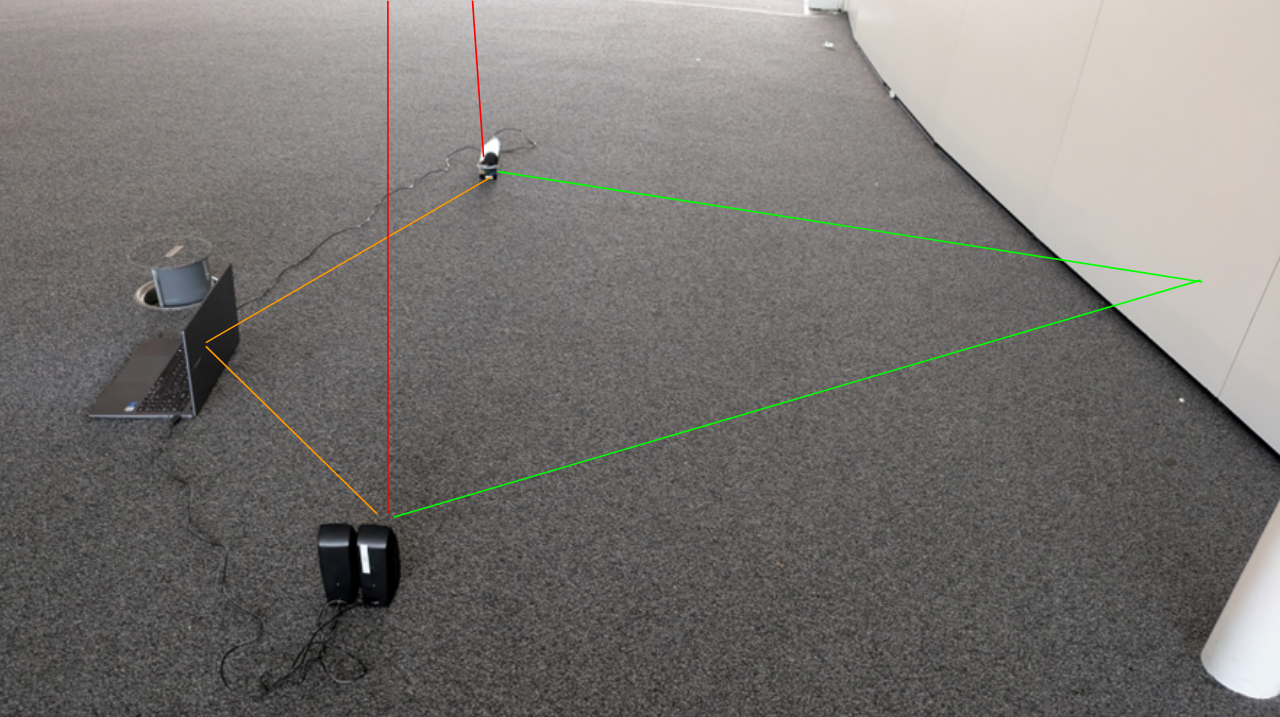
\includegraphics[width=0.70\textwidth]{figures/chap5_transmission/imag1.png}
    }
\end{figure}

The increased distance between the transmitter and receiver results in significant signal attenuation due to the exponential decay of acoustic energy, thereby reducing the Signal-to-Noise Ratio (SNR) and potentially increasing the Bit Error Rate (BER).
Despite these adverse conditions, the channel estimation performed using the methodology described in \Cref{ch:channel} successfully captured the multipath profile.

Analysis of the Impulse Response, detailed in \Cref{fig:trans_cir_pdp} in the appendix, reveals a sparse channel structure dominated by three primary components:
\begin{itemize}
    \item \textbf{Tap 1:} The direct path, carrying the highest energy.
    \item \textbf{Tap 2:} A short-delay reflection, likely attributable to the laptop screen or keyboard.
    \item \textbf{Tap 4:} A delayed component, corresponding to the reflection from the distant glass wall.
\end{itemize}

Following the strategy defined in the previous chapter, we applied a practical MMSE windowing technique to truncate the impulse response, retaining only these significant taps to minimize noise injection during equalization. The corresponding LMMSE report is available in \Cref{fig:trans_lmmse_report}.

\section{Image Transmission Challenges}

Transmitting image data introduces specific challenges compared to continuous data streams, primarily regarding temporal stability and data integrity.

\subsection{Signal Fragmentation}
The transmission of a high-resolution image requires a signal duration of several seconds.
In a real acoustic environment, the channel is potentially time-varying (e.g., due to movement or temperature fluctuations).
If the entire image were transmitted as a single block, the channel estimate obtained at the preamble could become stale by the end of the packet, leading to equalization errors.

To mitigate this, the image was fragmented into 10 independent frames.
Each frame carries its own preamble and training symbol, forcing a re-estimation of the channel for every segment.
This ensures that the equalization coefficients remain valid for the duration of the frame, adapting to any slow variations in the environment.

\subsection{Data Sensitivity and Formats}
We utilized the Bitmap (BMP) format for transmission.
Unlike compressed formats (e.g., JPEG), where a single bit error can destroy the entropy coding and render the image unreadable, Bitmaps are more resilient to payload errors.
However, they still rely on a critical \textbf{file header} to define dimensions and color depth.

\begin{remark}[The Header Problem]
    If the file header is corrupted by noise or deep fading, the receiver cannot reconstruct the pixel grid, resulting in a total failure to display the image.
    While our current implementation successfully retrieved the image (as shown in \Cref{fig:result_image}), the risk of header corruption suggests the need for robust protection.
\end{remark}

\begin{figure}[!ht]
    \centering
    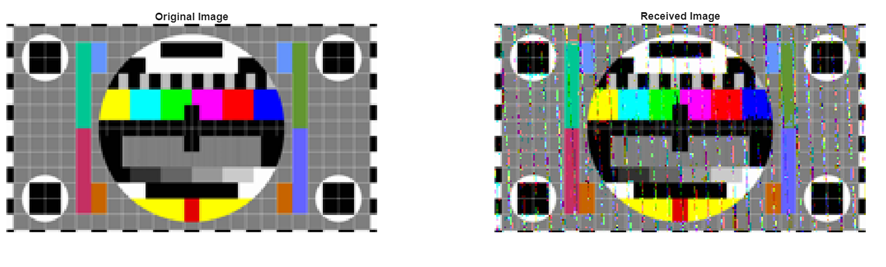
\includegraphics[width=0.85\textwidth]{figures/chap5_transmission/imag5.png}
    \caption[Transmission Results]{Comparison between the original transmitted test pattern and the received image. The system successfully recovered the color information despite the multipath environment, with a measured BER of \num{0.094}.}
    \label{fig:result_image}
\end{figure}

The visual result confirms the viability of the equalization scheme.
However, to ensure reliability in cases where the BER spikes, it is necessary to implement Forward Error Correction (FEC), particularly to protect critical metadata such as image headers.
This optimization is the subject of the following chapter.

\subsection{Peak-to-Average Power Ratio (PAPR) and Nonlinearities}
\label{sub:PAPR}

A significant drawback of the OFDM modulation used in this acoustic transmission is the high Peak-to-Average Power Ratio (PAPR), a characteristic that becomes particularly problematic when transmitting structured data like images. In our experiment, if the image data contains repetitive patterns—such as large areas of a single color in a BMP file—the transmitted symbols $A[k]$ become highly correlated. When these symbols are processed by the Inverse Fast Fourier Transform (IFFT), they may align in phase, resulting in constructive interference that produces large instantaneous power peaks.

The continuous-time baseband OFDM signal can be expressed mathematically as the sum of $N$ orthogonal subcarriers:
\begin{equation} \label{eq:ofdm_signal_papr}
    s(t) = \frac{1}{\sqrt{N}} \sum_{k=0}^{N-1} A[k] \E^{\I 2\pi k \Delta f t} \eqcomma \quad 0 \le t \le T \eqend
\end{equation}
The PAPR is defined as the ratio between the maximum instantaneous power and the average power of the signal:
\begin{equation} \label{eq:papr_formula}
    \text{PAPR}\{s(t)\} \doteq \frac{\max_{0 \le t \le T} |s(t)|^{2}}{\mathbb{E}\left[|s(t)|^{2}\right]} \eqend
\end{equation}

In a typical acoustic scenario, these power spikes are detrimental for several reasons. First, if the peaks exceed the linear dynamic range of the loudspeaker's power amplifier or the digital-to-analog converter (DAC), the signal is clipped, leading to severe nonlinear distortion. This clipping introduces "spectral regrowth," which generates out-of-band interference, but more critically, it creates in-band distortion. This effect manifests as an additional noise floor that degrades the constellation points, as seen in the spread of symbols in \Cref{fig:ch5_ber_performance} (a), and unlike Gaussian noise, it cannot be fully mitigated by the LMMSE equalizer alone.



To mitigate this effect during the Rolex Learning Center trials, the digital gain was backed off (Input Back-Off) to ensure the peaks remained within the linear region of the hardware. While this prevents nonlinear distortion, it simultaneously reduces the average signal power, leading to a lower Signal-to-Noise Ratio (SNR) at the receiver. This trade-off explains why certain frames exhibited higher BER despite successful channel estimation, as the system operated with reduced power margins to accommodate these PAPR spikes.